\documentclass [notitlepage] {article}
\usepackage[margin=1.0in,nohead,nofoot]{geometry}
\usepackage{url}
\usepackage{hyperref}
\usepackage{graphicx}
\usepackage{color}
\pagestyle{empty}
\newcommand\myurl[2]{\url{#1}}
\newcommand\email[1]{\href{mailto:#1}{\nolinkurl{#1}}}
\newcommand{\fixme}[1]{\textcolor{red}{FIXME: #1}\marginpar{\textcolor{red}{\textbf{F}}}}
%\renewcommand{\fixme}[1]{}


\title{CMS Software and Computing Performance Paper (Title TBD)}

\author{CMS Collaboration - Editors: K.Bloom and P.Elmer}


\begin{document}

\maketitle

\abstract{The specifications and performance of the CMS offline software
  and computing systems during Run 1 of the Large Hadron Collider are
  described.  Planned changes for Run 2 are also discussed.  Real abstract
  to be written later.  }

\section{Introduction}

\subsection {Physics goals} 

\begin{itemize}
\item describe quantitatively the scale required to reach physics goals
\item Higgs~\cite{CMSHIGGS} as possible example physics problem, should (briefly!) run through all the S\&C needs to do the physics analysis.  (At the very least, Higgs provides the example of quick turnaround of physics -- when was the last data taken before 4/7/12 Higgs announcement?)  Is there another physics problem that has some contrasting requirements?  Another physics requirement -- must get results out fast due to competition and great community interest!
\end{itemize}

\subsection{The Large Hadron Collider and the CMS detector}

\begin{itemize}
\item Scale and requirements of the LHC
\item Scale and requirements of the CMS detector
\item Event size, Pile-Up (e.g. effect on multiplicities, etc.)
\end{itemize}

\subsection{Software and Computing System} 

\begin{itemize}
\item Describe the major limitations and challenges in building the S\&C system
\item requirements of distributed development and distributed computing facilities:
\item These include: large group of code developers whose are ultimately novice coders, wide geographical distribution of developers, highly distributed computing resources too, newfangled grid system that had to be shaken down, very distributed and ultimately novice-coder analysts! (I think we should be covering analysis in here too)...what else do we need to add to this list?
\end{itemize}

Goals of software and computing:

\begin{itemize}
\item Software development model must incorporate the work of many geographically distributed coders
\item Software must run on all necessary architectures, must be robust against potentially fragile computing facilities
\item Software needs to be able to run at a scale needed to turn around results quickly
\item Computing must run the software at the sufficient scale
\item Computing must make the best use of all available resources
\item Computing must make the data and computing resources available to all analysts
\item In general, software and computing should never limit the rate of the production of physics results and papers (``factory'' latency) Do we have a way of demonstrating this actually happened?
\end{itemize}


\section{Software Applications} 
Describe what are we trying to do with the computing:
\begin{itemize}

\item Trigger (how much of this is ``us''?  HLT?)
% CHEP 2013 	"The CMS High Level Trigger" D. Troncino
% https://cms-mgt-conferences.web.cern.ch/cms-mgt-conferences/conferences/pres_display.aspx?cid=1085&pid=7050

% CHEP12 "The CMS High Level Trigger System: Experience and Future
% Development" A. Sparatu
% https://cms-mgt-conferences.web.cern.ch/cms-mgt-conferences/conferences/pres_display.aspx?cid=665&pid=4520

\item Reconstruction
% CHEP13 "The Role of Effective Event Reconstruction in the Higgs Boson Discovery at CMS", S. Krutelyov
% https://cms-mgt-conferences.web.cern.ch/cms-mgt-conferences/conferences/pres_display.aspx?cid=1085&pid=7258

\item Analysis

\item MC simulation
% CHEP13 - there is both a fastsim talk and a fullsim talk, but I think
% we combined these. I'm confused by what we have in Cinco, will double
% check on CHEP13 site (I'm one of the track coordinators for that CHEP track)

\item Calibration/alignment
% CHEP13 "Alignment and calibration of CMS detector during collisions at LHC" R.Castello
% https://cms-mgt-conferences.web.cern.ch/cms-mgt-conferences/conferences/pres_display.aspx?cid=1085&pid=7170

\item I considered also things like data management here, but that strictly speaking isn't something needed to get a physics result, which I think is what this section is about.  Anything missing from the list?
\end{itemize}


\section{Software Implementation}
\begin{itemize}

\item Software development model

\item Framework architecture 
% Perhaps some of the text can come from the paper about the new
% framework evolution:
% CHEP13 "Stitched Together: Transitioning CMS to a Hierarchical Threaded Framework" C. Jones
% https://cms-mgt-conferences.web.cern.ch/cms-mgt-conferences/conferences/pres_display.aspx?cid=1085&pid=7110
% or perhaps there are older CHEP papers.

\item Software architecture and evolution

\item ``Performance'' numbers (code base size, number of developers, etc.) 
over time, major releases

% CHEP10 "The CMS Reconstruction Software" D. Lange
% https://cms-mgt-conferences.web.cern.ch/cms-mgt-conferences/conferences/pres_display.aspx?cid=462&pid=2346

\item Software and Release validation
% CHEP13 "The Rise of the Build Infrastructure" G.Eulisse
% https://cms-mgt-conferences.web.cern.ch/cms-mgt-conferences/conferences/conf_display.aspx?cid=1085

% CHEP 10 "Release Strategies: CMS approach for Development and Quality
% Assurance", E. Sexton-Kennedy
% https://cms-mgt-conferences.web.cern.ch/cms-mgt-conferences/conferences/pres_display.aspx?cid=462&pid=2344

\item Evolution with architectures (32bit/64bit, compilers)
% Various ACAT/CHEP presentations from P.Elmer, M.Kortelainen

\item CPU and I/O optimization?
% Various ACAT/CHEP presentations from P.Elmer, M.Kortelainen

\item Documentation?
% Surely we have documentation?
% CHEP12 "Developing CMS software documentation system" M. Stankevicius
% https://cms-mgt-conferences.web.cern.ch/cms-mgt-conferences/conferences/pres_display.aspx?cid=665&pid=4506

\end{itemize}


\section{Computing Implementation} 

\subsection{Distributed computing infrastructure}

% CHEP12 "Trying to Predict the Future - Resource Planning and Allocation
% in CMS" P. Kreuzer
% https://cms-mgt-conferences.web.cern.ch/cms-mgt-conferences/conferences/pres_display.aspx?cid=665&pid=4582

% CHEP10 "Experience with the CMS Computing Model from commissioning to
% collisions" D. Bonacorsi
% https://cms-mgt-conferences.web.cern.ch/cms-mgt-conferences/conferences/pres_display.aspx?cid=462&pid=2306

% CHEP10 "Monitoring the Readiness and Utilization of the Distributed CMS
% Computing Facilities during the first year LHC running" J. Hernandez
% https://cms-mgt-conferences.web.cern.ch/cms-mgt-conferences/conferences/pres_display.aspx?cid=462&pid=2332
% Note that we don't currently have monitoring in here as an explicit
% topic.  But it probably needs to be discussed in operations, at the very least.

% CHEP10 "CMS Distributed Computing Integration in the LHC sustained
% operations era" C. Grandi
% https://cms-mgt-conferences.web.cern.ch/cms-mgt-conferences/conferences/pres_display.aspx?cid=462&pid=2264

From the very start, CMS planned on having a distributed computing
infrastructure.  While HEP collaborations have historically relied on a
single large computational resource located at the host laboratory for
virtually all of their data processing and storage needs, and while a
single facility would have ultimately been more efficient to operate, it
was not considered feasible to ask the nations of the LHC experimental
collaborations to contribute funds for a computing center at CERN.
Instead, each nation has established domestically owned and operated sites
that contribute to the LHC experiments' computing needs.  These sites,
distributed around the world, have given greater prominence to the LHC
experiments within their participating nations, which has led to greater
funding and more engagement from local computing experts, who would not
have had a chance to participate had all the computing been done at CERN.
CMS has successfully leveraged this local expertise to improve the
experiment's computing systems and their operation.

The CMS distributed computing infrastructure is a tiered set of computing
sites connected through networks that follows the MONARC
model~\cite{MONARC}. The computing infrastructure is organized in a
hierarchy starting with CERN facility, called Tier 0 (T0), at its origin.
On the next level, seven regional computing centers called Tier-1 (T1)
sites form the backbone of the system, followed by Tier-2 (T2) and Tier-3
(T3) sites at universities and/or research institutes.

Sites at each tier in the hierarchy are responsible for performing certain
workflows, and the sites are configured to support those particular
workflows.  \fixme{In fact, the description of the workflows might take
  place in the ``applications'' section, we'll see, but keep some
  information here for now.}  The T0 site is responsible for data recording
and first-pass (``prompt'') data reconstruction, and also for performing
calibrations that are needed for the reconstruction.  Prompt reconstruction
starts 48 hours after events have been recorded to incorporate updated
calibrations.  The production of calibration constants is described in
Section~\ref{sec:constants}.  All events are stored in the RAW format on
tape at the T0 site.  \fixme{We'll need to be sure that RAW etc. are
  defined earlier on; this sounds like software.}  The T0 facility thus
needs substantial processing and storage resources.  At the end of Run 1,
the CMS T0 facility had \fixme{Get all the T0 parameters!}.

The primary workflows at T1 sites are the simulation of events and the
re-reconstruction of both detector and simulation events.  Simulation is a
processing-intensive workflow that requires little or no input data, but
has large output data.  Re-reconstruction of the data and simulation
samples is performed when changes to reconstruction algorithms and/or
calibrations are sufficiently different from those of the prompt
reconstruction to have a significant impact on understanding the physics of
the LHC collisions.  The re-reconstruction workflow also requires
substantial processing resources, and both the input and output data sizes
are large.  In addition, the T1 sites are responsible for maintaining a
second archived copy of the data in RAW format, so that between the T0 and
T1 sites, there are two tape copies of every event.  To fulfill all of
these missions, T1 sites must host processing, disk and tape resources.
CMS operated seven T1 sites during Run 1, hosted by Germany, Spain, France,
Italy, Taiwan, the United Kingdom and the United States.  At the end of the
run, the aggregated Tier 1 resources were \fixme{Get all the T1 parameters!
  Do we discuss relative sizes of sites?  Mention the hosting
  institutions?}

T2 sites are also responsible for some simulation workflows, and also for
analysis of data and simulation samples by physics users; no user analysis
takes place at T0 or T1.  The input datasets for analysis are distributed
to the sites in advance, and then jobs seeking to analyze a particular
dataset are sent to a site that hosts the data.  While the input data for
analysis is typically large, the output is usually several orders of
magnitude smaller, as users reduce and refine the data to meet their
specific interests and needs.  \fixme{Give some typical sizes for these?
  Does such a thing exist?  Will it be elsewhere?}  T2 sites do no archival
storage, so are only required to deploy disk and processing resources.  In
Run 1, there were about fifty T2 sites, which in aggregate provided
\fixme{Get all the T2 parameters!}.  An important distinction between T2
sites and those at T0 and T1 is that the former only offer business-hour
site support and are unattended in between.

T3 sites are owned and managed by individual institutes, at a support level
of their choosing, and they execute workflows of their choosing.  T3 sites
are most often used for final-stage data analysis by the local users of the
site.  There is no set configuration for the T3 sites.

For all of the workflows, the input data must reside at the site where the
workflow is executed.  In many cases the data needs to be transferred from
another site.  All sites are interconnected via dedicated or general
purpose scientific networks. The original design separated the T2 sites
into groups that were associated with and connected to only one T1. During
LHC Run 1, the strength and reliability of the networks allowed for a more
flexible setup, realizing a full-mesh network topology where every T2 site
is connected to every T1 site and every other T2 site, as shown in
Figure~\ref{fig:distributed_topology}.  The full-mesh network allowed for
much greater ease in data movement, as a given T2 site could receive data
from a large number of potential source sites, and greater flexibility in
operations, as it was easier to move a particular dataset to a given site
so that the necessary workflows could be performed there.

\begin{figure}
\begin{center}
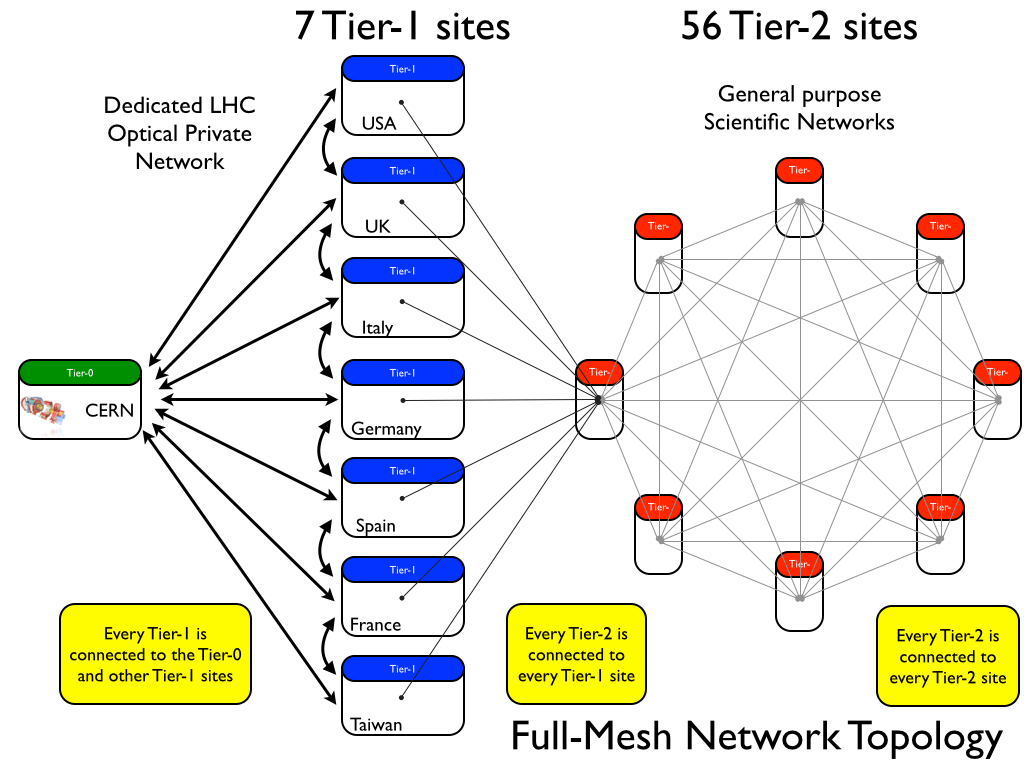
\includegraphics[width=.5\textwidth]{figs/distributed_topology}
\end{center}
\caption{The tiered CMS computing infrastructure showing the Tier-0, Tier-1 and Tier-2 levels interconnected with dedicated or general purpose scientific networks in a full-mesh network topology.
  \label{fig:distributed_topology}}
\end{figure}

The network between the sites is the backbone of the CMS computing
infrastructure, as its operation relies on transferring files among the
sites for access. The network between the T0 and T1 sites is the dedicated
LHC Optical Private Network (LHCOPN).~\fixme{Does this get a
  reference?}. The T2 sites are connected through general purpose
scientific networks in their host countries. The main data flows can be
separated into archiving and serving. Archiving is tape based where related
files are grouped by physics content on separate sets of tape cartridges
(known as tape families) to optimize writing, recall, and
recycling. Serving is disk based. The main data flows are as follows:

\begin{itemize}
\item {\bf T0 $\to$ T1}: RAW data recorded by the detector is recorded at
  T0 and stored on tape as a ``cold'' backup replica. The RAW is
  distributed across the T1's via the LHCOPN network links and archived on
  tape. The tape replica at the T1's can be recalled at any time and is
  called the custodial replica. The mass storage system at the T1's also
  provides caching capabilities and the files from the current year of data
  taking are kept cached.

\item {\bf T1 $\to$ T1}: Both RAW and simulated data are reconstructed for
  analysis on the T1 level. This requires especially strong I/O
  capabilities. The resulting AOD holds the minimum amount of information
  needed for analysis and is archived at the Tier-1 that stored the
  custodial tape copy of the input data.

\item {\bf T1 $\to$ T2}: As data of all formats is archived at T1 sites,
  which do not allow access by regular analysis users, any dataset that an
  analysis user requires must be transferred to a T2 site.  T2 disk is
  logically separated into managed portions for common samples and
  unmanaged areas for files belonging to individual users and physics
  groups.

\item {\bf T2 $\to$ T1}: The output of the simulation of a specific physics
  process at a T2 site is consolidated at a Tier-1 site where it is stored
  on tape.
\end{itemize}

An important distinction between T2 sites and those at T0 and T1 is that
the latter were used by a small number of operators for centrally-organized
production tasks.  The T2 sites were used by physicists throught the
collaboration in a ``chaotic'' mode.  Thousands of users might submit jobs
to any given site.  To maintain scalability of management, users do not
directly log in to computers at the sites, but instead submit jobs from
their local login machine through grid technologies~\cite{thegrid}.  A
computing grid is an infrastructure that allows different administrative
domains to share access to services, processors and storage with a select
set of users and groups of users. The computing clusters that are members
of a grid provide a uniform environment for user batch jobs, even if each
cluster has some unique local configuration.  As a result, any user job
can, in principle, be executed at any site on the grid with little user
customization required.  Users of the grid resources are issued credentials
that can be attached to a batch job when it is submitted to a resource;
these credentials allow for the tracking of jobs back to individual users.

The technology used to operate grid sites is known as ``middleware,'' as it
has a role that is somewhere between the actual hardware that operates at a
site and the software that is run by user applications.  CMS sites operated
using three different varieties of middleware.  Most sites in Europe and
Asia used the Euopean Grid Infrastructure (EGI)~\cite{EGI} middleware,
while a few sites in Northern Europe used the Advanced Resource Connector
(ARC)~\cite{ARC} middleware.  Sites in the Western Hemisphere were part of
the Open Science Grid (OSG)~\cite{OSG}.  All sites were members of the
Worldwide LHC Computing Grid (WLCG)~\cite{WLCG}, which developed a number
of common applications for the LHC experiments.  In practice, CMS developed
a number of applications that ran on top of the middleware, to make it
easier for users to access information about the data catalogue and
calibration constants that needed to be passed to the computers that
executed the jobs.  These are described in Section\fixme{Probably the
  Workflow Execution section, but need to see how this rolls out}.

This physical infrastructure of the computing sites and the wide area
network, plus the middleware infrastructure of the grid, requires a large
number of services and applications that make it useful for the CMS
workflows.  These are described in the remainder of this section.
Section~\ref{sec:corecomponents} describes the services needed for the
creation and distribution of calibration constants, data transfers, data
management, software distribution, and job submission.
Section~\ref{sec:compops} discusses the operations model for the
infrastructure, and the tools needed to monitor sites and jobs.
Section~\ref{sec:workflow} describes the management of both production and
analysis workflows.


\subsection{Core computing services}
\label{sec:corecomponents}

\subsubsection{Constants creation and distribution}
\label{sec:constants}
% PCL, Frontier

% CHEP10 "Alignment & calibration experience under LHC data-taking
% conditions in the CMS experiment" R. Mankel
% https://cms-mgt-conferences.web.cern.ch/cms-mgt-conferences/conferences/pres_display.aspx?cid=462&pid=2324

% CHEP12 "Handling of time-critical Conditions Data in the CMS experiment -
% Experience of the first year of data taking" G. Govi
% https://cms-mgt-conferences.web.cern.ch/cms-mgt-conferences/conferences/pres_display.aspx?cid=665&pid=4571

% CHEP12  "Comparison of the Frontier Distributed Database Caching System with NoSQL Databases" D. Dykstra
% https://cms-mgt-conferences.web.cern.ch/cms-mgt-conferences/conferences/pres_display.aspx?cid=665&pid=4418

% CHEP12 "CMS experience with online and offline Databases" A. Pfeiffer
% https://cms-mgt-conferences.web.cern.ch/cms-mgt-conferences/conferences/pres_display.aspx?cid=665&pid=4444

% CHEP12 "Operational Experience with the Frontier System in CMS"
% https://cms-mgt-conferences.web.cern.ch/cms-mgt-conferences/conferences/pres_display.aspx?cid=665&pid=4540

% CHEP10 "Time-critical database condition data handling in the CMS
% experiment during the first data taking period" S. Di Guida
% https://cms-mgt-conferences.web.cern.ch/cms-mgt-conferences/conferences/pres_display.aspx?cid=462&pid=2300

% CHEP10 "CMS Online Database experience with first data" M. Janulis
% https://cms-mgt-conferences.web.cern.ch/cms-mgt-conferences/conferences/pres_display.aspx?cid=462&pid=2310


\subsubsection{Data transfers}
% PhEDEx

% CHEP13 "The CMS Data Management System" N. Magini
% https://cms-mgt-conferences.web.cern.ch/cms-mgt-conferences/conferences/pres_display.aspx?cid=1085&pid=7057

% CHEP12 "CMS Data Transfer operations after the first years of LHC
% collisions" R. Kaselis
% https://cms-mgt-conferences.web.cern.ch/cms-mgt-conferences/conferences/pres_display.aspx?cid=665&pid=4537

% CHEP12 "Performance studies and improvements of CMS Distributed Data
% Transfers", J. Flix
% https://cms-mgt-conferences.web.cern.ch/cms-mgt-conferences/conferences/pres_display.aspx?cid=665&pid=4536

% CHEP10 "Large Scale Commissioning and Operational Experience with Tier-2
% to Tier-2 Data Transfer Links in CMS" J. Letts
% https://cms-mgt-conferences.web.cern.ch/cms-mgt-conferences/conferences/pres_display.aspx?cid=462&pid=2265

% CHEP10 "Improving CMS data transfers among its distributed Computing
% Facilities" N. Magini
% https://cms-mgt-conferences.web.cern.ch/cms-mgt-conferences/conferences/pres_display.aspx?cid=462&pid=2323

% CHEP12 "From toolkit to framework - the past and future evolution of
% PhEDEx" T. Wildish
% https://cms-mgt-conferences.web.cern.ch/cms-mgt-conferences/conferences/pres_display.aspx?cid=665&pid=4552


\subsubsection{Data management}
% DBS
% CHEP10 "Data Aggregation System, an information retrieval on demand over
% relational and non-relational distributed data sources." V. Kuznetsov
% https://cms-mgt-conferences.web.cern.ch/cms-mgt-conferences/conferences/pres_display.aspx?cid=462&pid=2317


\subsubsection{Software distribution}
% CVMFS (and predecessors)

\subsubsection{Submission tools}
% glite, HTCondor_g, glide-in


\subsection{Computing operations and monitoring}
\label{sec:compops}

\subsubsection{Operations model}

\subsubsection{Site monitoring}

\subsubsection{Job monitoring}


\subsection{Workflow execution}
\label{sec:workflow}

\subsubsection{Production workflow management}
% WMAgent
% CHEP12 "The CMS workload management system" S. Wakefield
% https://cms-mgt-conferences.web.cern.ch/cms-mgt-conferences/conferences/pres_display.aspx?cid=665&pid=4454

% CHEP12 "A new era for central processing and production in CMS"
% E. Fajardo Hernandez
% https://cms-mgt-conferences.web.cern.ch/cms-mgt-conferences/conferences/pres_display.aspx?cid=665&pid=4402

% CHEP12 "CMS resource utilization and limitations on the grid after the
% first two years of LHC collisions" K. Bloom
% https://cms-mgt-conferences.web.cern.ch/cms-mgt-conferences/conferences/pres_display.aspx?cid=665&pid=4542

% CHEP10 "Measuring and Understanding Computing Resource Utilization in
% CMS" J. Letts
% https://cms-mgt-conferences.web.cern.ch/cms-mgt-conferences/conferences/pres_display.aspx?cid=462&pid=2268


\subsubsection{User analysis workflows}
% CRAB

% CHEP12 "CMS Analysis Deconstructed" S. Malik
% https://cms-mgt-conferences.web.cern.ch/cms-mgt-conferences/conferences/pres_display.aspx?cid=665&pid=4399

% CHEP12 "Maintaining and improving of the training program on the analysis
% software in CMS" S. Malik
% https://cms-mgt-conferences.web.cern.ch/cms-mgt-conferences/conferences/pres_display.aspx?cid=665&pid=4570

% CHEP10 "Perspective of User Support for the CMS Collaboration" S. Malik
% https://cms-mgt-conferences.web.cern.ch/cms-mgt-conferences/conferences/pres_display.aspx?cid=462&pid=2263

% CHEP10 "A tour of the CMS Physics Analysis Model" B. Hegner
% https://cms-mgt-conferences.web.cern.ch/cms-mgt-conferences/conferences/pres_display.aspx?cid=462&pid=2309

% CHEP10 "CMS distributed analysis infrastructure and operations:
% experience with the first LHC data" E. Vaandering
% https://cms-mgt-conferences.web.cern.ch/cms-mgt-conferences/conferences/pres_display.aspx?cid=462&pid=2338

% CHEP10 "Design and early experience with promoting user-created data in
% CMS" M. Giffels
% https://cms-mgt-conferences.web.cern.ch/cms-mgt-conferences/conferences/pres_display.aspx?cid=462&pid=2293






\section{Anticipated Evolution for Run 2}
\begin{itemize}
\item Multithreaded framework
%CHEP12 "Study of a Fine Grained Threaded Framework Design" C. Jones
% https://cms-mgt-conferences.web.cern.ch/cms-mgt-conferences/conferences/pres_display.aspx?cid=665&pid=4396

%CHEP12 "Multi-core processing and scheduling performance in CMS"
%J. Hernandez
% https://cms-mgt-conferences.web.cern.ch/cms-mgt-conferences/conferences/pres_display.aspx?cid=665&pid=4365

%CHEP10 "Multicore-aware applications in CMS" C. Jones
% https://cms-mgt-conferences.web.cern.ch/cms-mgt-conferences/conferences/pres_display.aspx?cid=462&pid=2342

\item Software engineering efforts
%CHEP12 "Development and Evaluation of Vectorised and Multi-Core Event
%Reconstruction Algorithms within the CMS Software Framework" D. Piparo
% https://cms-mgt-conferences.web.cern.ch/cms-mgt-conferences/conferences/pres_display.aspx?cid=665&pid=4546

\item Evolution of tiered computing model
% CHEP12 "Evolution of the Distributed Computing Model of the CMS
% experiment at the LHC" C. Grandi
% https://cms-mgt-conferences.web.cern.ch/cms-mgt-conferences/conferences/pres_display.aspx?cid=665&pid=4347

\item Use of data federations, changes in data distribution
%CHEP12 "Implementing data placement strategies for the CMS experiment
%based on a popularity mode" D. Giordano
% https://cms-mgt-conferences.web.cern.ch/cms-mgt-conferences/conferences/pres_display.aspx?cid=665&pid=4443
\item Efforts on opportunistic resources
% CHEP12 "Controlled overflowing of data-intensive jobs from oversubscribed
% sites" I. Sfiligoi
% https://cms-mgt-conferences.web.cern.ch/cms-mgt-conferences/conferences/pres_display.aspx?cid=665&pid=4419
\end{itemize}

\section{Conclusion}
Would be good to get back to the physics -- discuss cases where we got results out quick (Higgs), turned around new samples quickly, got new releases or calibrations out fast.  These are ultimately the measures of our success!  Or put another way, here is where we should clearly emphasize that we’ve met some of the goals described earlier.



\bibliographystyle{unsrt}
\bibliography{references}

\end{document}

